\documentclass[11pt, oneside]{article}   	% use "amsart" instead of "article" for AMSLaTeX format
\usepackage{geometry}                		% See geometry.pdf to learn the layout options. There are lots.
\geometry{letterpaper}                   		% ... or a4paper or a5paper or ... 
%\geometry{landscape}                		% Activate for for rotated page geometry
%\usepackage[parfill]{parskip}    		% Activate to begin paragraphs with an empty line rather than an indent
\usepackage{graphicx}				% Use pdf, png, jpg, or eps� with pdflatex; use eps in DVI mode
								% TeX will automatically convert eps --> pdf in pdflatex		
\usepackage{amssymb}
\usepackage{amsmath}
\usepackage{parskip}

\title{Cosine s+t quickly}
%\author{The Author}
\date{}							% Activate to display a given date or no date
\graphicspath{{/Users/telliott_admin/Dropbox/Tex/png/}}

\begin{document}
\section*{Cosine s+t quickly}
%\maketitle
%\section{}
%\subsection{}
\Large
Suppose we consider a right triangle, with one of the angles labeled $s$.  We can scale this triangle to any size we like, and all the different scaled triangles will be similar to each other, having the third angle complementary to $s$, with sum equal to $\pi/2$.

Now construct another right triangle containing angle $t$, and scale it so that the base adjacent to angle $t$ is just as long as the hypotenuse of the triangle containing angle $s$, and then draw them next to each other as shown:
\begin{center} 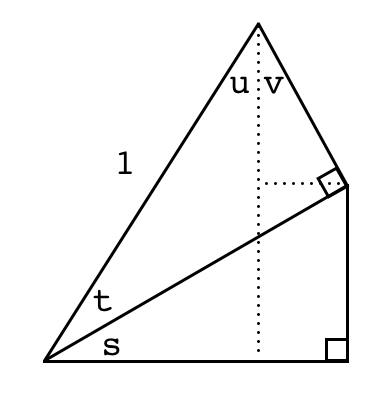
\includegraphics [scale=0.5] {sum_angle2.png} \end{center}
I have also scaled the joined triangles so that the hypotenuse of the second triangle has unit length.

Our crucial insight is to draw vertical and horizontal dotted lines as shown.  Since the vertical line makes a right angle with the base, we have that:
\[ s + t + u = \frac{\pi}{2} =  t + u + v \]
\[ s = v \]

Since I already know the result I am looking for, I write 
\[ \cos s + t = \cos s \cos t - \sin s \sin t \]

By $\cos s + t$ we really mean $\cos (s + t)$, but have left off the parentheses.

Our goal is to verify this eternal truth, using the diagram.  We add some labels to the sides of the triangles and substitute into the above equation, using the figure for reference:
\begin{center} 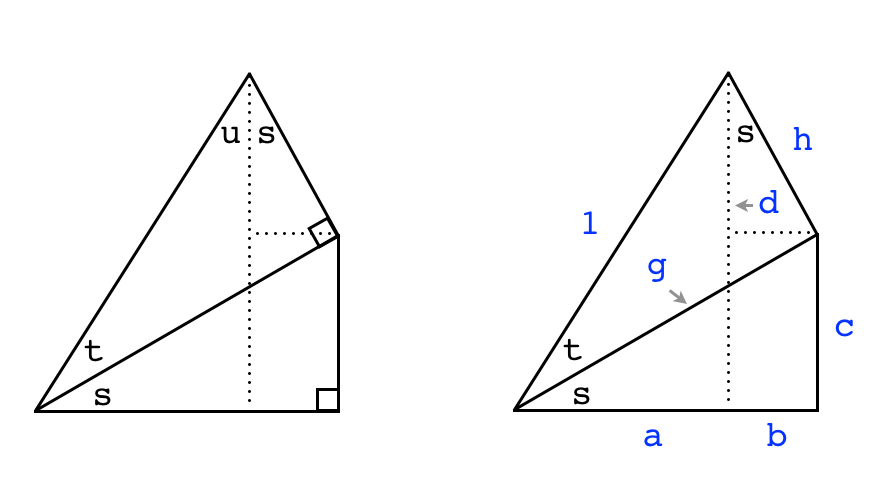
\includegraphics [scale=0.5] {sum_angle.png} \end{center}
From the figure
\[ \cos s = \frac{a+b}{g}; \ \ \ \cos t = \frac{g}{1}; \ \ \ \cos s \cos t = a + b \]
\[ \sin s = \frac{b}{h}; \ \ \ \sin t = \frac{h}{1}; \ \ \ \sin s \sin t = b \]
\[ \cos s + t = a = (a + b) - b \]
And from our calculation:
\[ \cos s \cos t - \sin s \sin t = (a + b) - b\]
Q.E.D.

As a quick check we can ask what happens to the formula 

\[ \cos s + t = \cos s \cos t - \sin s \sin t \]

when $t = 0$.  Then the first term is the cosine of $s$, and the second term is equal to $0$.

\subsection*{extension to minus}
The first extension is to the difference $\cos s - t$.  We have
\[ \cos s + (-t) = \cos s \cos (-t) - \sin s \sin (-t) \]
Now, recall that $\cos -t = \cos t$ and $\sin -t = - \sin t$.  

(Although it's not a proof, just visualize what happens near $\theta = 0$ and $\theta$ becomes negative).  Or, remember that the sine is an odd function $f(x) = - f(-x)$ and that the cosine is an even function---cosine is symmetric about the $y$-axis.  Thus
\[ \cos s -t = \cos s \cos t + \sin s \sin t \]
I like this form because it's easy to verify that if $s=t$ then we have $\cos 0 = 1 = \cos^2 s + \sin^2 s = 1$, which is the most famous trig identity.

\subsection*{extension to sine}
Referring back to the diagram (and again, with our goal clearly in mind)
\[ \sin s =  \frac{c}{g} \ \ \ \  \cos t = \frac{g}{1} \ \ \ \  \sin s \cos t = c  \]
\[ \sin t = \frac{h}{1} \ \ \ \  \cos s = \frac{d}{h} \ \ \ \ \sin t \cos s = d \]
But 
\[ \sin s + t = c + d =  \sin s \cos t +  \sin t \cos s \]

Using the even/odd function rules, we get

\[ \sin s - t = c + d =  \sin s \cos t -  \sin t \cos s \]

You should commit all the formulas to memory.  They can easily be used to derive other formulas, like the double-angle formula.

\end{document}  